\subsection{Préparation}

\begin{figure}[H]
    \begin{center}
    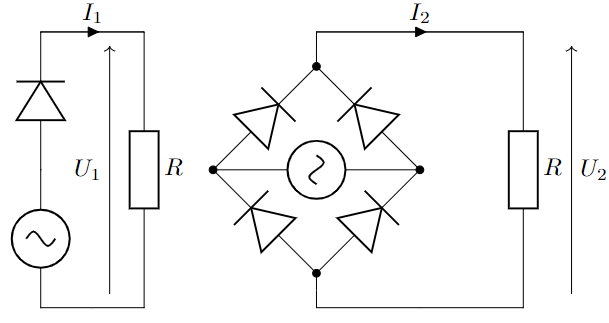
\includegraphics[scale=0.5]{images/4.png}
    \caption{Redresseur de tension}
    \end{center}
\end{figure}

\underline{$\star$ Rappel :}

$V_{eff}=\sqrt{2}*V_{max}$
$V_{max}=\frac{V_{pp}}{4}$
$V_{moy}=\frac{V_{max}}{2\pi}$

Voici l'allure des composants $U_1$, $U_2$, $I_1$ et $I_2$, sachant que $R=1k\Omega$ et $V_{PP}=5V$ :


\begin{figure}[H]
    \begin{center}
    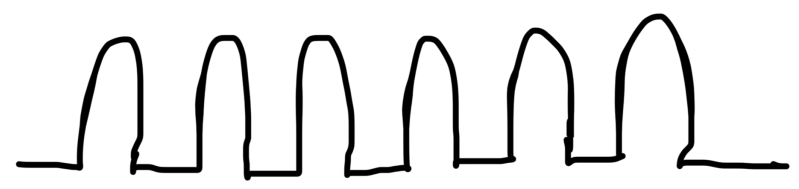
\includegraphics[scale=0.5]{images/boucle1.png}
    \caption{Allure de $U_1$ et $I_1$}
    \end{center}
\end{figure}

\begin{figure}[H]
    \begin{center}
    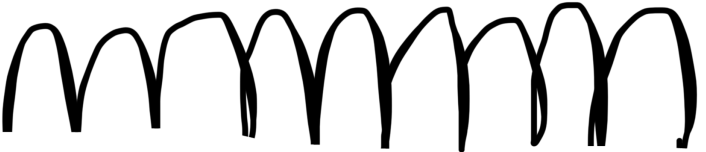
\includegraphics[scale=0.5]{images/boucle2.png}
    \caption{Allure de $U_2$ et $I_2$}
    \end{center}
\end{figure}

\newpage
Calculons ensuite les valeurs moyennes et efficaces de $U_1$ et $U_2$ :

\[V{pp}=5V\]
\[V_{moy1}=\frac{V_{max1}}{2\pi} \simeq 0.39V\]
\[V_{eff1}=\frac{V_{max1}}{\sqrt{2}}= 0.884V\]

\[V_{max2}=2V_{moy1}\simeq0.78V\]
\[V_{eff2}=\sqrt{2}*1.25=0.884V\]


La valeur moyenne de $U_1$ est de $0.39V$ et la valeur efficace est de $0.884V$. Pour $U_2$, la valeur moyenne est de $0.78V$ et la valeur efficace est de $0.884V$.

\newpage
\subsection{Redresseur mono-alternance}

Nous avons réalisé le premier circuit et avons mesuré la tension aux bornes de la résistance $R$ appelée $U_1$. Voici l'oscillogramme correspondant :

\begin{figure}[H]
    \begin{center}
    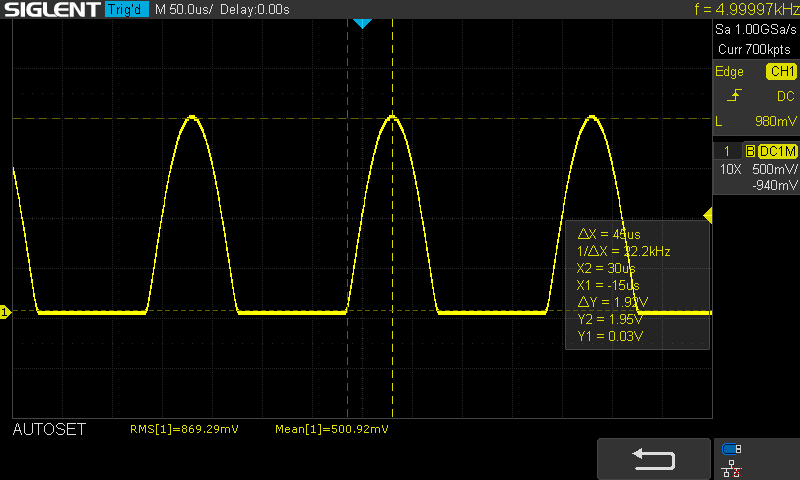
\includegraphics[scale=0.5]{images/Oscillo/SDS00006.png}
    \caption{Oscillogramme de la tension $U_1$ avec $R=1K\Omega$.}
    \end{center}
\end{figure}
Nous pouvons voir sur la capture d'écran précédente que la tension moyenne est de $869.29mV$ et la tension efficace est de $500.92mV$ . Nous avons donc des résultats proches de ceux calculés précédemment.

Ensuite, nous avons ajouté un condensateur de $1\mu F$ en parallèle de la résistance $R$ et avons mesuré la tension aux bornes de ce dernier. Voici l'oscillogramme correspondant :

\begin{figure}[H]
    \begin{center}
    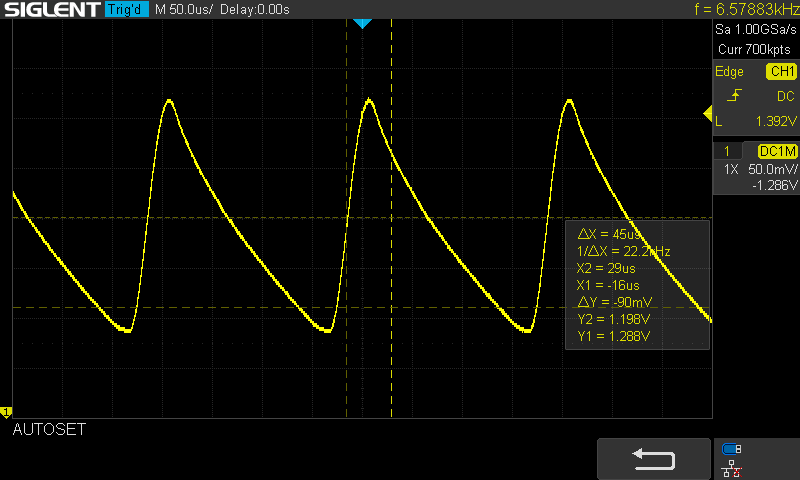
\includegraphics[scale=0.5]{images/Oscillo/SDS00003.png}
    \caption{Oscillogramme de la tension $U_1$ avec $R=1k\Omega$ et $C=1\mu F$.}
    \end{center}
\end{figure}

Nous pouvons déduire de la courbe précédente que des sortes de pics se forment, ce qui est dû au condensateur qui se charge et se décharge.

Après quoi, nous avons modifié la résistance pour une résistance de $10k\Omega$ et avons mesuré la tension aux bornes de la résistance. Voici l'oscillogramme correspondant :
\begin{figure}[H]
    \begin{center}
    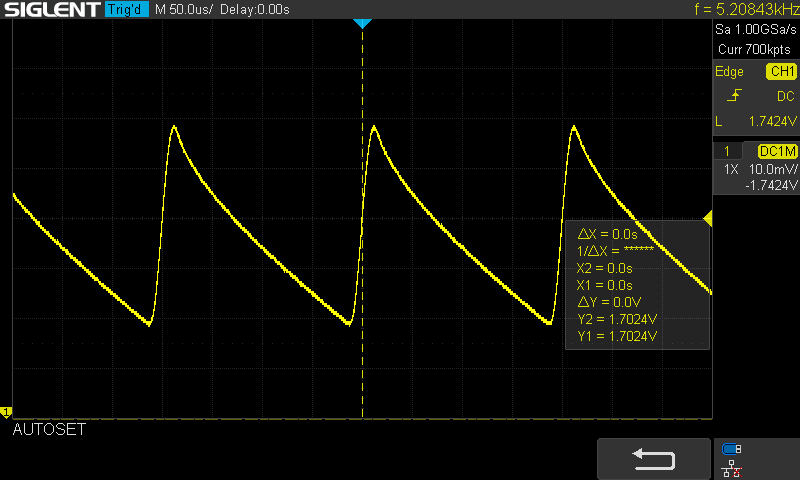
\includegraphics[scale=0.4]{images/Oscillo/SDS00004.png}
    \caption{Oscillogramme de la tension $U_1$ avec $R=10k\Omega$ et $C=1\mu F$.}
    \end{center}
\end{figure}


